\documentclass{beamer}
% Class options include: notes, notesonly, handout, trans,
%                        hidesubsections, shadesubsections,
%                        inrow, blue, red, grey, brown

% Theme for beamer presentation.
\usepackage{beamerthemesplit} 
% Other themes include: beamerthemebars, beamerthemelined, 
%                       beamerthemetree, beamerthemetreebars  

\title[The Practicality of Prompt Engineering]{The Practicality of Prompt Engineering}
\author{Isaac Liu}
\date{\today}

\usepackage{graphicx} % http://ctan.org/pkg/graphicx
\usepackage{amsmath}
\usepackage{geometry}
\usepackage{amsfonts}
\usepackage[english]{babel}
\usepackage{amssymb}
\usepackage{graphicx}
\usepackage{float}
\usepackage{hyperref}
\usepackage{multirow}
\usepackage{pdflscape}
\usepackage{caption}
\usepackage{pdflscape}
\usepackage{outlines}
\usepackage{subcaption}

\usepackage{framed}

\usepackage{tabularx, booktabs}

\usepackage{standalone}

\usepackage[autostyle, english = american]{csquotes}
\MakeOuterQuote{"}

\usepackage{comment}

\hypersetup{
    colorlinks=true,
    linkcolor=white,
    filecolor=black,      
    urlcolor=black,
}

\setbeamertemplate{navigation symbols}{}

\begin{document}
    \begin{frame}
        \frametitle{The Practicality of Prompt Engineering}
        \begin{itemize}
            \scriptsize
            \item Cost (length/complexity, financial) efficacy of prompt engineering
            \item 100 programmatic conversations - math (GSM8K), creative writing
            \item Contribution - quantification, statistical tests, old + new models
            \item Statistically significant improvements (paired tests): GSM8K all, creative writing GPT-4 manual CoT, zero-shot CoT
            \item Zero-Shot CoT cheaper, more powerful than few-shotting that came before, complicated techniques that came after
            \item TD3 to GPT-4 - GSM8K gains down, CW gains up
            \item A few pennies per 1K tokens - cheap GSM8K, expensive CW improvements
        \end{itemize}
        \begin{figure}[h]
            \begin{subfigure}[h]{0.4925\textwidth}
                \centering
                %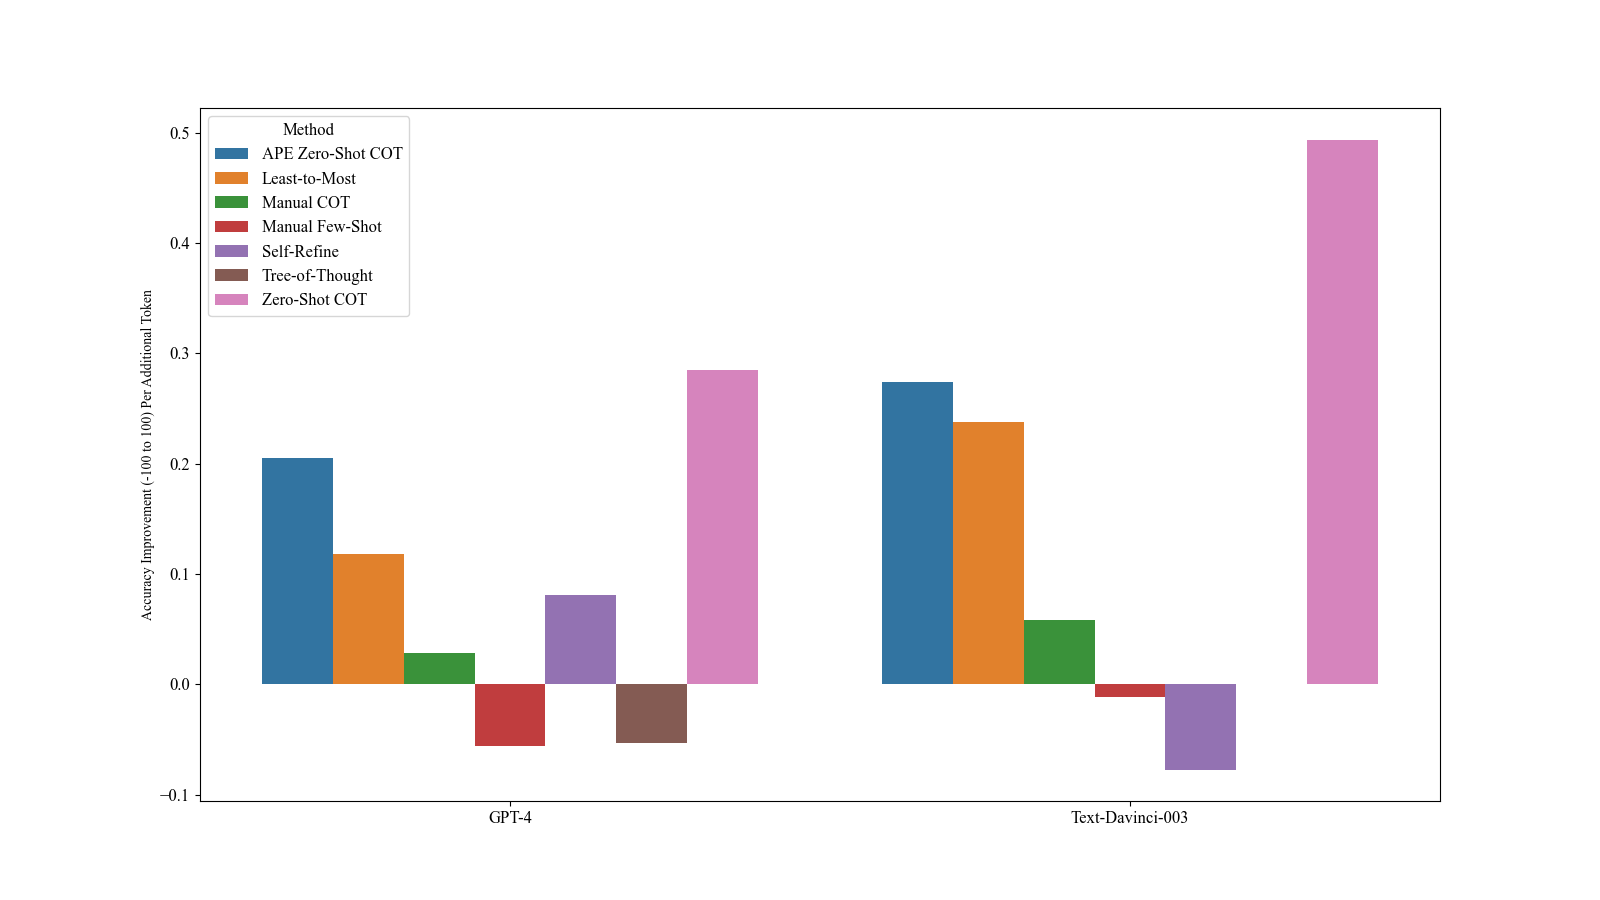
\includegraphics[width=0.95\hsize]{../Output/gsm8k_change_in_accuracy_quality_per_change_in_conversation_length.png} 
                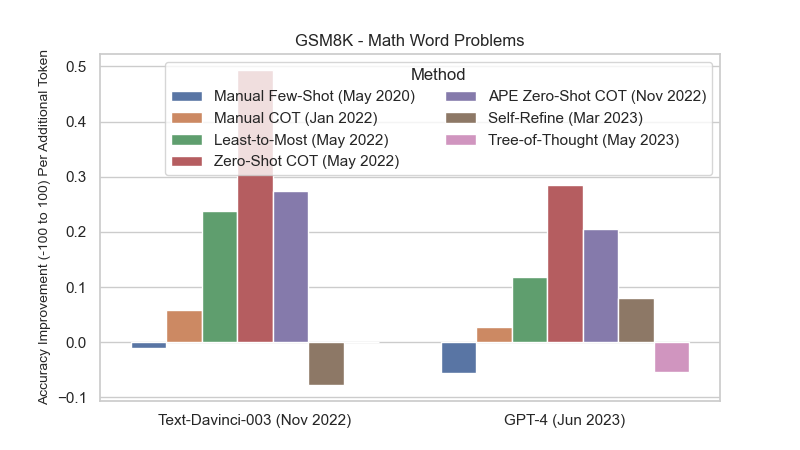
\includegraphics[width=1.1\hsize]{../Output/gsm8k_change_in_accuracy_quality_per_change_in_conversation_length_sorted_by_technique_age.png} 
                %\subcaption*{GSM8K Math Word Problems}
            \end{subfigure}
            %\hfill
            \begin{subfigure}[h]{0.4925\textwidth}
                \centering
                %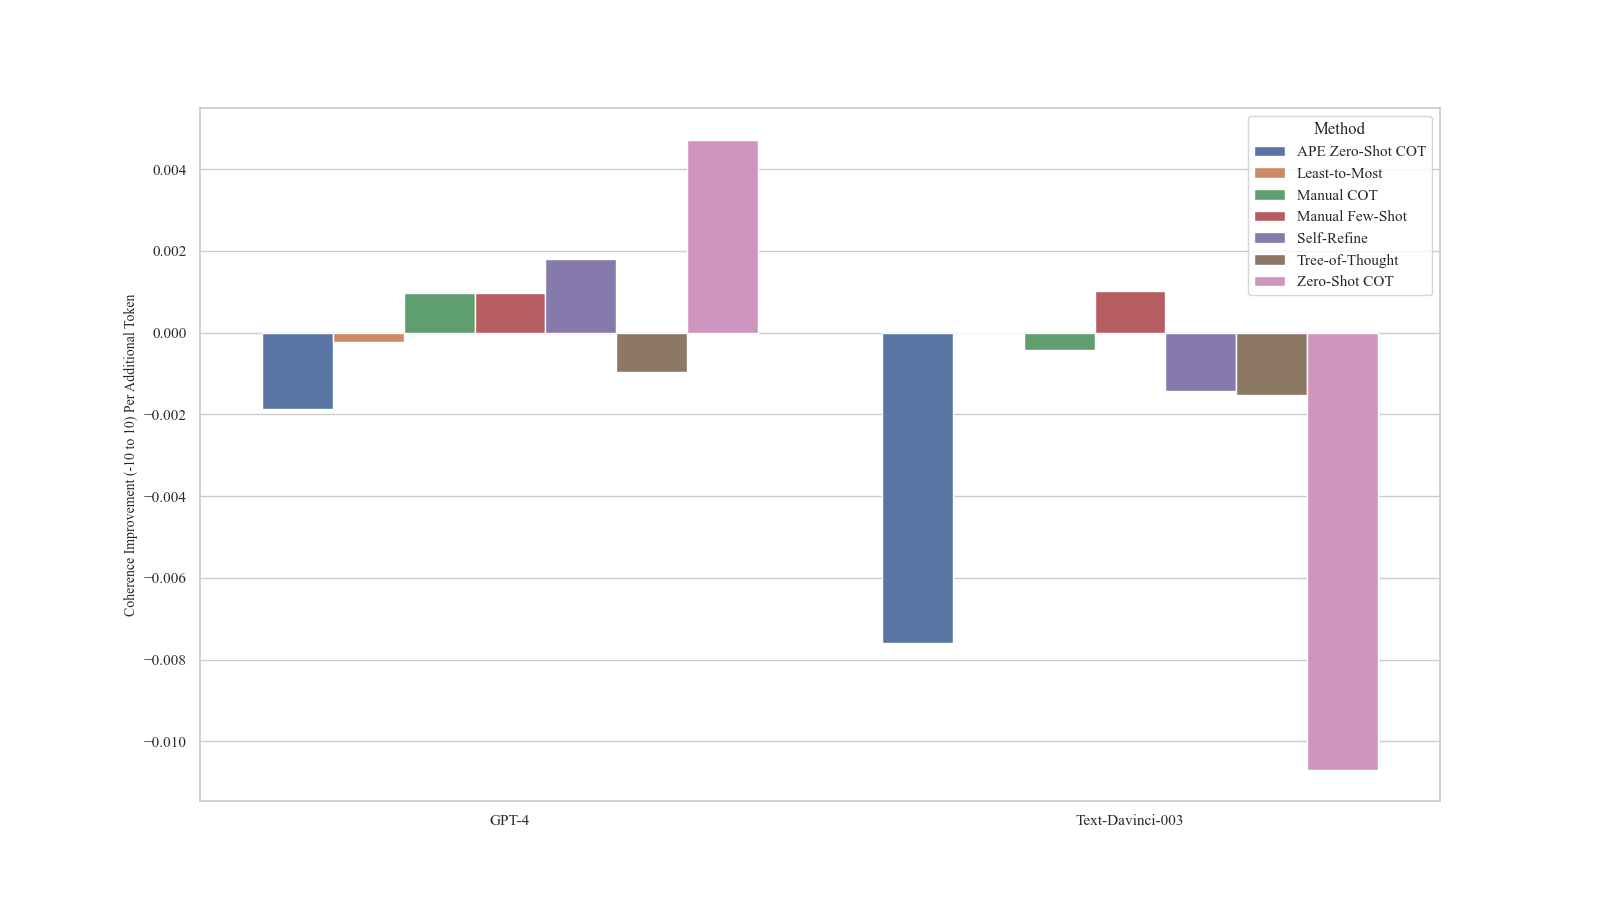
\includegraphics[width=0.95\hsize]{../Output/cw_change_in_accuracy_quality_per_change_in_conversation_length.png}
                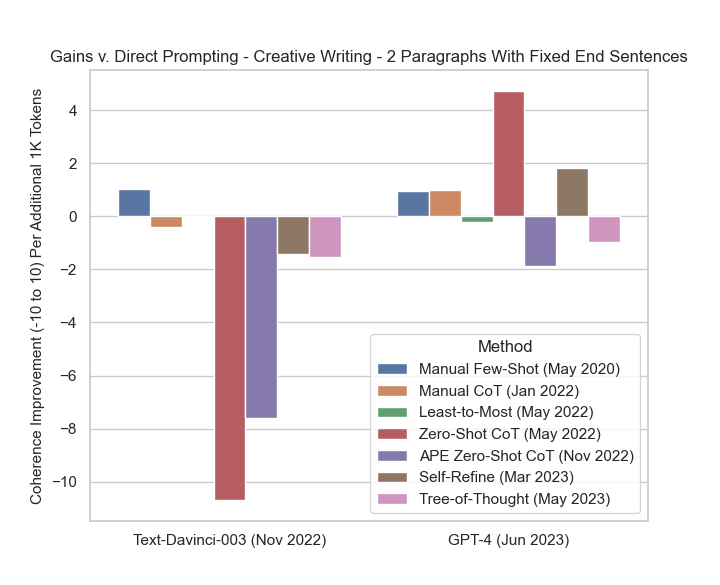
\includegraphics[width=1.1\hsize]{../Output/cw_change_in_accuracy_quality_per_change_in_conversation_length_sorted_by_technique_age_transformed.png}
                %\subcaption*{Fixed-End-Sentence Creative Writing}
            \end{subfigure}
        \end{figure}
    \end{frame}
\end{document}
